Pro řádné otestování realizovaného rozšíření bylo využito jednotkových a integračních testů. Testy jsou umístěny ve
složce \mintinline{text}{src/spec} a jejich výstup po kompilaci pak ve složce \mintinline{text}{spec}. Jsou spouštěny s
pomocí komunitního \textit{test runner} atom-jasmine3-test-runner, který byl zvolen na základě provedené rešerše \ref
{vyber-komunitniho-test-runner}. Testy tak mají (stejně jako kód samotného rozšíření) plný přístup k API Atomu a mohou
pracovat s webovými APIs.

Pro přehlednost byl při tvorbě testů použit takzvaný AAA vzor – jednoduchý vzor, kdy je každý test členěn do třech
částí. V první (\textit{arrange}) části jsou dle \cite{aaa} nejprve inicializovány objekty a očekávané výstupy. V další
(\textit{act}) části je pak dle \cite{aaa} zavolána testovaná metoda či funkce. V poslední (\textit{assert}) části je
nakonec dle \cite{aaa} ověřeno, že testovaná metoda či funkce funguje dle očekávání.

Především jednotkové testy pak používají \textit{mock}, \textit{stub} a \textit{spy} objekty. Pro zjednodušení jejich
tvorby byla využita populární knihovna Sinon.JS, která se na tuto oblast dle \cite{sinon} specializuje a funguje s
libovolným frameworkem pro jednotkové testování. Knihovna Sinon.JS je dle \cite{sinon} dostupná pod permisivní
open-source licencí (mimo jiné) z npm \cite{npm} a nabízí také \textit{types} pro TypeScript.

Tyto testovací objekty pak spolu s použitím interfaces a \textit{inversion of control} techniky \textit{dependency
injection} ve zdroji rozšíření umožňují docílit (mimo jiné) izolace chování tříd. Další pomocné interfaces jsou
vytvořeny pro abstrakci funkcionality vybraných tříd z Atom API (jejichž instance jsou dostupné v globální proměnné
\mintinline{text}{atom}). Například třída \mintinline{text}{Workspace} z Atom API má totiž dle \cite{atom-docs} desítky
metod, z nichž realizované rozšíření jich využívá pouhé jednotky. Díky vlastním interfaces jako jsou například
\mintinline{text}{WorkspaceItemManager} nebo \mintinline{text}{WorkspaceObserver} je tak docíleno \textit{low coupling}.
Jednou komplikací při vytváření \textit{mock} objektů na základě interfaces v jazyce TypeScript je, že \textit{mock}
objekty není možno vytvářet s pomocí generujících funkcí/metod Sinon.JS. Je tomu z důvodu absence typových informací
(mezi něž interfaces patří) v JavaScript výstupu (typové informace jsou dle \cite{ts-docs} volitelně přidány pouze jako
samostatné \textit{types} soubory pro využití v dalším TypeScript kódu).

V průběhu realizace bylo dále využito jednoduchých uživatelských testů, kdy byla nově přidávaná funkcionalita vyzkoušena
na WooWoo zdrojích existujících studijních textů autorem práce na operačním systému Windows 10 a vedoucím práce na
Linuxové distribuci Arch Linux.

Pro automatizaci jednotkových a integračních testů bylo využito platformy pro kontinuální integraci GitHub Actions.
GitHub Actions umožňují dle \cite{gh-actions} tvorbu vlastních \textit{actions}, které lze dále v oficiálním \uv
{obchodě} sdílet s komunitou. Jednou z takto dostupných \textit{actions} je Setup Atom \cite{github-action-setup-atom},
která umožňuje jednoduché nastavení Atomu pro použití v (nejen) tomto nástroji pro kontinuální integraci. Setup Atom dle
\cite{github-action-setup-atom} umožňuje použití nejnovější stabilní verze Atomu nebo jedné z vývojových verzí. Dále dle
\cite{github-action-setup-atom} umožňuje použití konkrétní verze Atomu (tato funkcionalita byla přidána na podnět autora
této práce). Díky těmto možnostem tak jde docílit zajištění korektního fungování na všech \textit{minor} verzích Atomu
mezi nejstarší testovanou verzí a nejnovější stabilní verzí bez nutnosti testování na všech těchto \textit{minor}
verzích (to platí dokud nevyjde nová \textit{major} verze a za předpokladu, že jsou řádně dodržována pravidla
semantického verzování).

Minimální takto podporovaná verze Atomu byla stanovena na 1.54, což byla nejnovější verze v době začátku realizace.
Testy jsou v kontinuální integraci spouštěny na nejnovějších verzích operačních systémů macOS, Ubuntu a Windows 10.
Dále je kontinuální integrace využita pro automatickou kontrolu sestavení, kontrolu formátování (za pomoci nástroje
Prettier), provedení statické analýzy (za pomoci nástroje ESLint) a vytvoření produkčního \textit{package}. Průběh
kontinuální integrace je ilustrován na obrázku \ref{testovani-ci}.

\begin{figure}\centering
    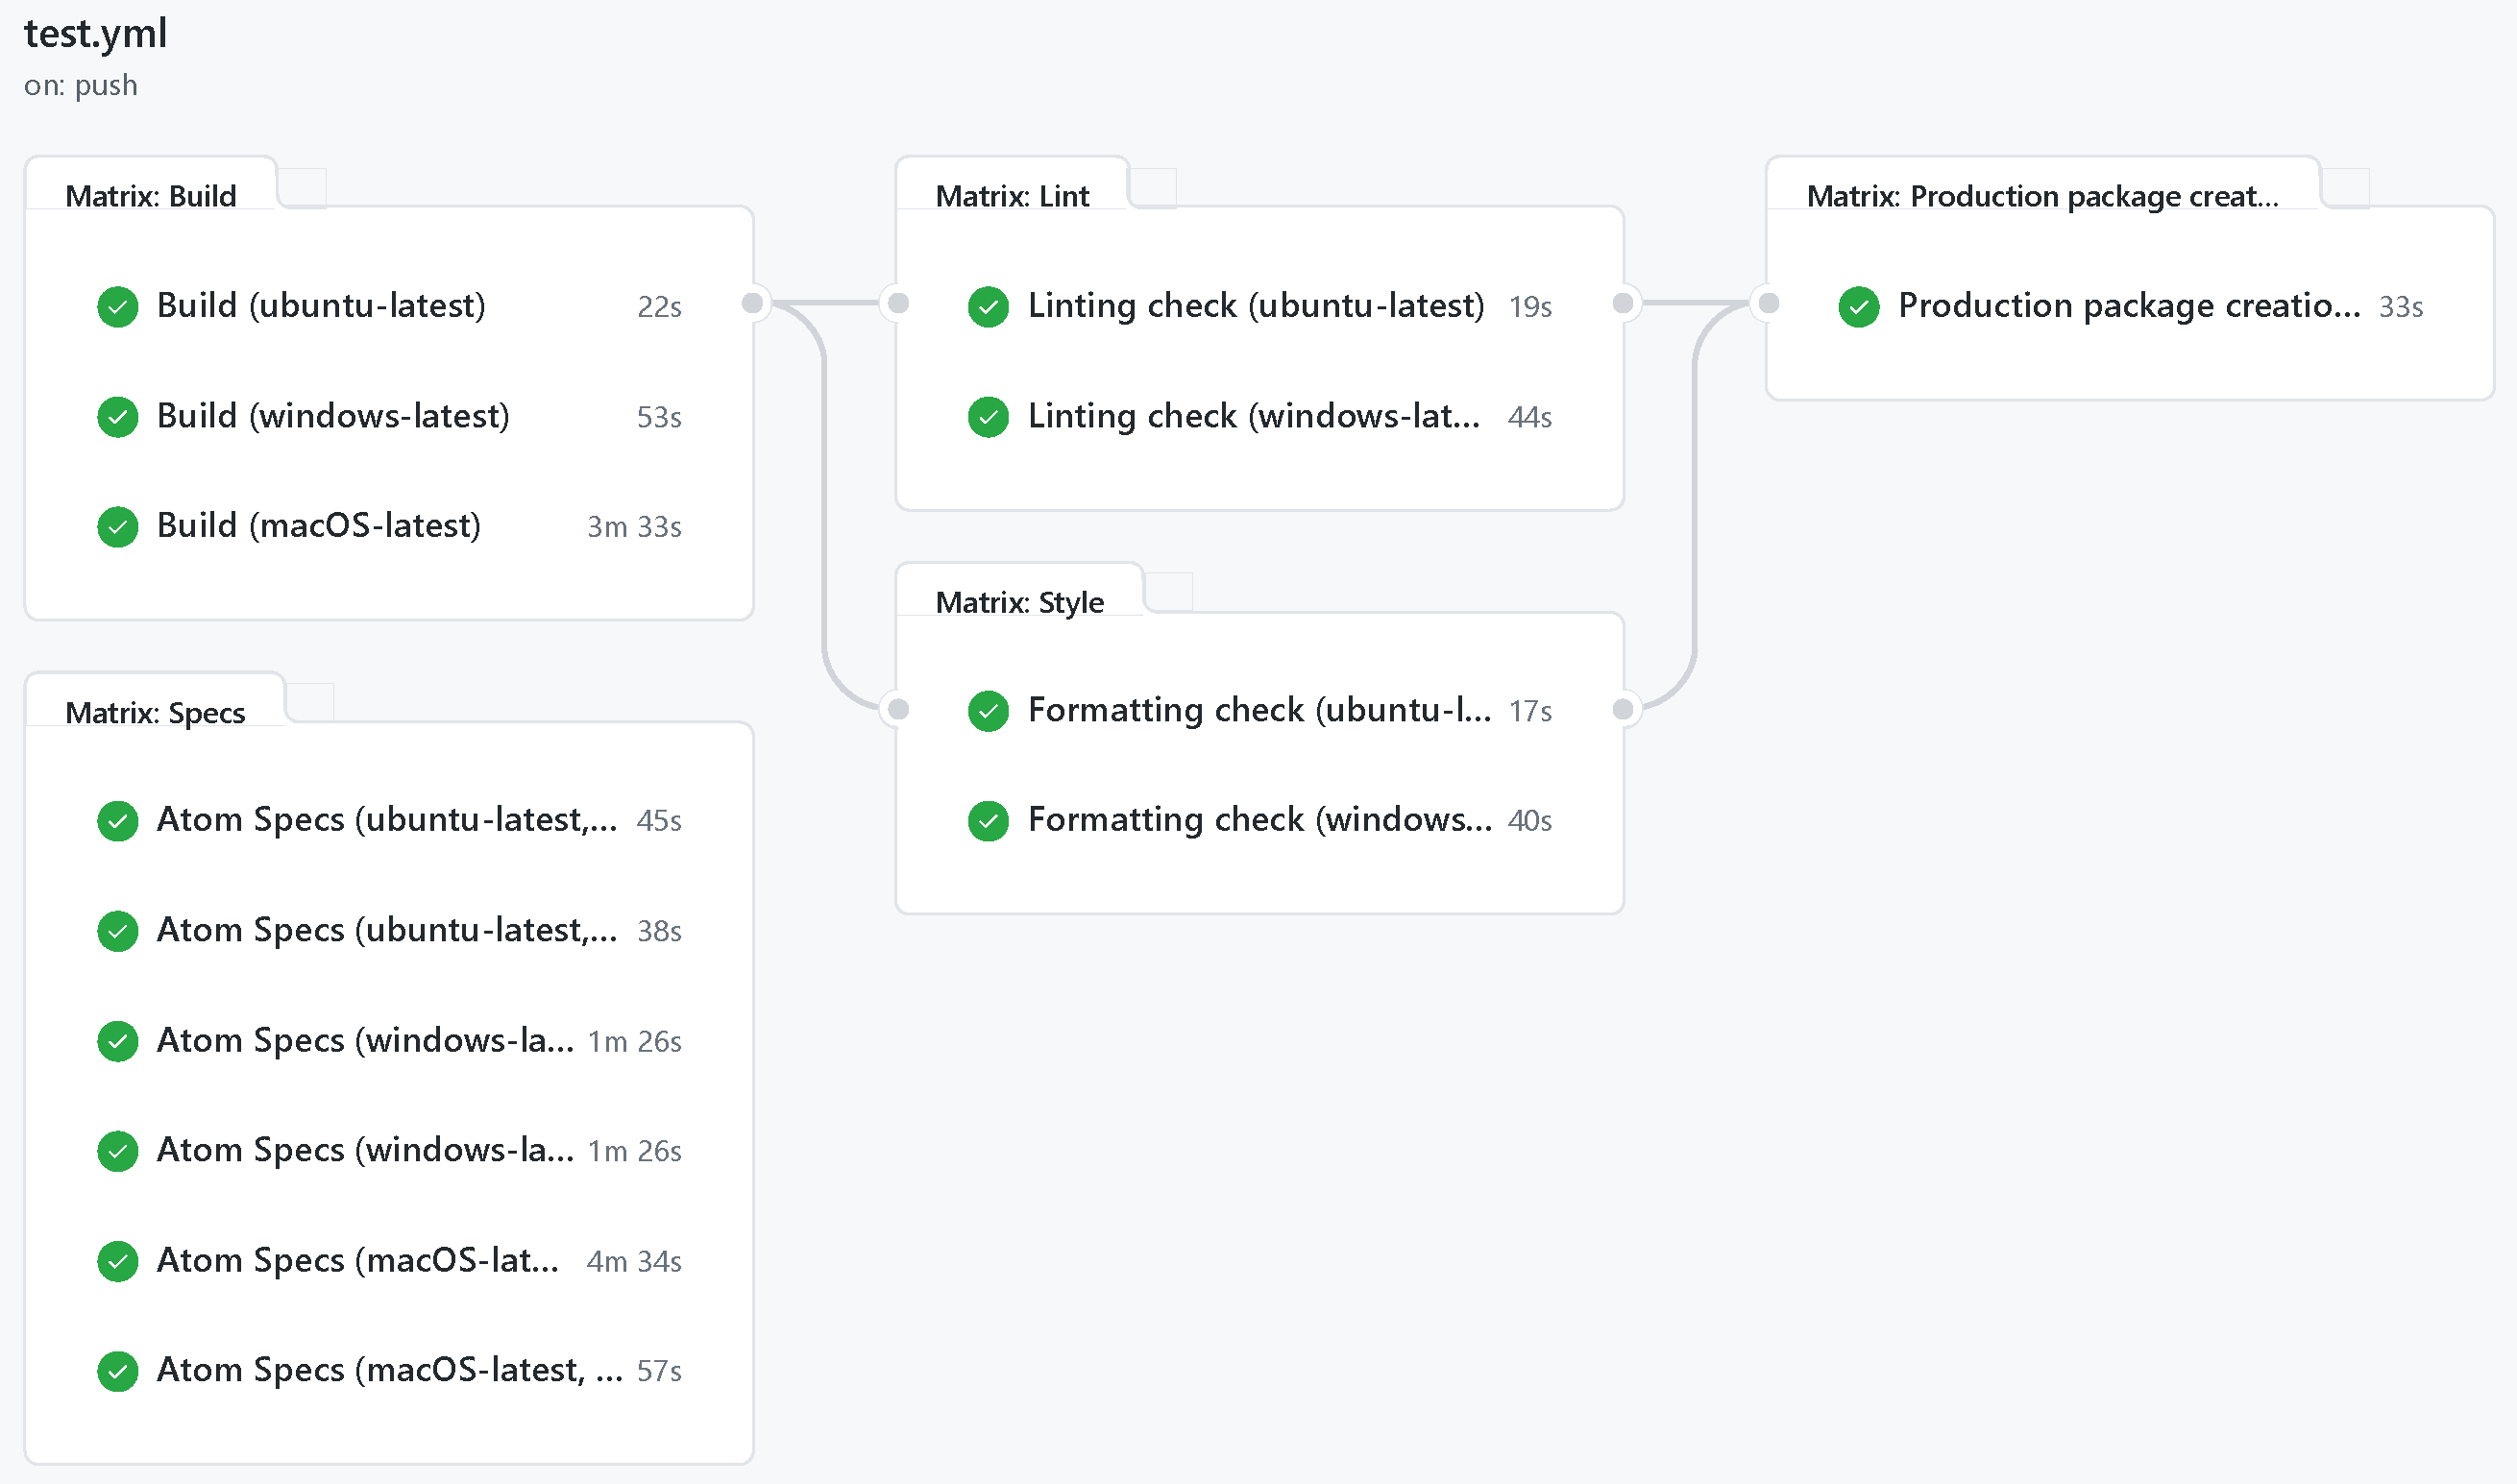
\includegraphics[width=1.0\textwidth]{content/realizace/testování-ci}
 	\caption[GitHub Actions \textit{workflow}]{Úspěšný běh GitHub Actions \textit{workflow}}
    \label{testovani-ci}
\end{figure}
